\chapter{Introdução}

\section{Motivação}

Organizar os procedimentos de um processo sempre nos traz vantagens. Apesar de no processo de implantação de um sistema, o mesmo burocratizar o processo, com o tempo temos o retorno da dedicação para a inserção dos dados. Com um certo volume de dados, é possível estruturar informações que num processo manual são difíceis de serem enxergadas. Assim, é possível depender menos das pessoas que organizam o processo, pois o legado de informações não estará mais somente na mente de alguns, mas sim documentado nos dados do sistema.

Além de colaborar na organização, também haverá uma grande colaboração no tempo gasto na gestão. Lidar com muitos papéis e confiar na mente humana para guardar informações, não é uma alternativa muito segura devido ao fato que as pessoas sempre estão sujeitas a sair do processo e levar contigo a experiência obtida. Experiência essa que faz com que os procedimentos sejam executados de forma mais eficiente. Entretanto, com um sistema inteligente, é possível auxiliar e tornar mais ágil a execução das tarefas.


\section{Problema}

começar de forma mais genérica
De acordo com funcionários ligados ao o setor de pós graduação da UFBA, entrevistados a fim de um maior entendimento do cenário, apesar das semelhanças estruturais, a pós graduação gerida de forma diferencia da graduação. FULANO afirma que devido ao fato de não ter a mesma visibilidade, não tem acesso aos mesmos recursos de gestão acadêmica da graduação. O professores não executam somente atividades dentro da sala de aula, também tem diversas outras ocupações no setor. E muitos procedimentos realizados extra classe ainda se encontram sendo realizados de forma manual, estando mais vulnerável ao erro ou até mesmo à violação do processo. Também ocorre um grande desperdício de tempo pelos professores e gestores da área, devido ao diversos processos ainda realizados de forma manual, sem a devida documentação. Segundo FULANO, também entrevistado, esse tempo perdido implica numa redução da eficiência na sala de aula, pois o professor acaba por ter menos tempo disponível para o planejamento das atividades, o que gera impactos negativos aos alunos.


\section{Objetivos} %<o que deve ser feito/entregue>

quebrar em geral e específicos
Devido aos muitos processos sendo resolvidos de forma manual, propõe-se com solução um sistema moderno, arquitetado para ter funcionamento na web e com um módulo mobile, a fim de fornecer informações de forma rápida e eficiente para os professores através de notificações, já que o acesso à internet móvel é comum entre os possíveis usuários do sistema em questão.
O principal requisito para o sistema seria dispor recursos para reduzir o tempo desperdiçado pelos professores durante as atividades extra classe.


\section{Metodologia} %<como será feito | como resolver o problema apontado inicialmente>


%<analise de literatura | design | implementação | validação>
Baseando-se nas tecnologias gratuitas em alta no cenário atual do desenvolvimento web, dispomos de algumas opções eficientes para a implementação da solução. Dentre as possibilidades, considerando a facilidade para futura manutenção e continuidade do projeto, tende-se a optar por uma tecnologia popular. Como linguagem de programação, adota-se o PHP. A escolha é fundamentada de acordo com a pesquisa da RedMonk de 2015 \cite{Grafico-RedMonk} , que evidencia o uso das linguagens de programação de acordo com as discussões no StackOverflow e repositórios no GitHub. É possível constatar a popularidade do PHP no cenário atual com o gráfico da pesquisa citada, na qual o PHP é apresentado na terceira colocação, apenas atrás do lider JavaScript e do segundo colocado, o Java.

\begin{figure}
	\label{fig:graficoRedmonk}
	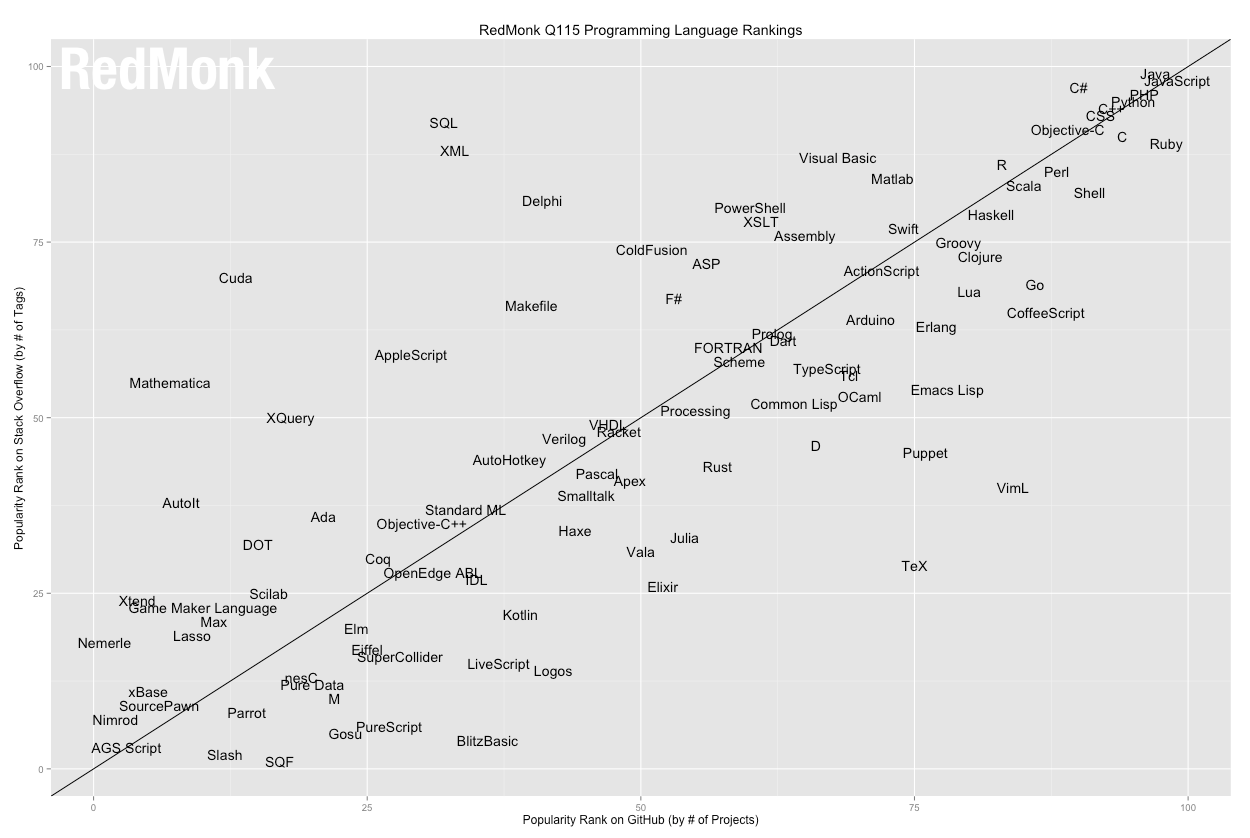
\includegraphics[width=1\textwidth]{img/grafico_redmonk}
	\caption{Ranking das liguagens de programação no Stack Overflow e Github}
\end{figure}


Ainda assim, para compor a interface do dado projeto, também ocorrerá o uso do líder JavaScript de forma intensa, provendo o elo com o as informações gerenciadas pelo PHP.


Entretanto, não seria inteligente desenvolver um sistema completo sem o auxílio de um framework. Dentre os frameworks disponíveis para PHP, hoje o destaque está com o Laravel, que se encontra no topo dentre os mais utilizados no momento. 


A WebHostFace, uma empresa de hospedagem, compilou várias estatísticas para criar um infográfico mostrando os frameworks PHP mais populares de 2015. Utilizando informações sobre os próprios clientes, o Google Trends, estatísticas de repositórios do GitHub e a pesquisa do SitePoint “Best PHP Frameworks 2015”, a WebHostFace elaborou o seguinte infográfico: 

\begin{figure}
	\label{fig:graficoWebhostface}
	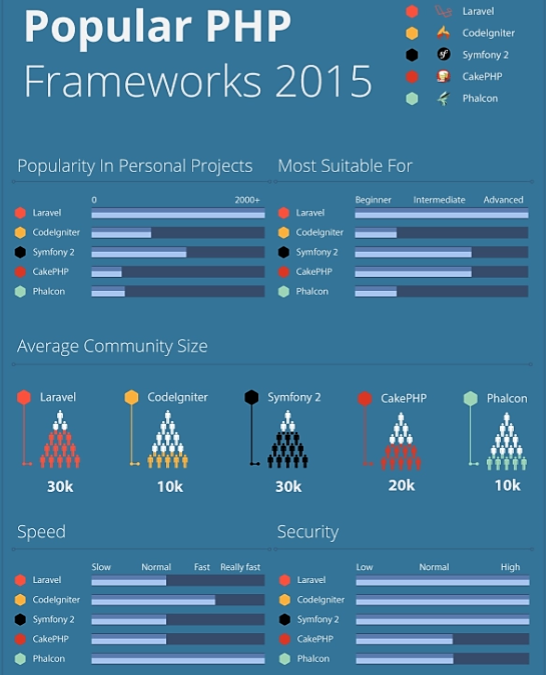
\includegraphics[width=1\textwidth]{img/infografico_webhostface}
	\caption{Infográfico da WebhostFace, exibindo a popularidade dos Frameworks PHP em 2015}
\end{figure}

Como pode ser verificado no gráfico \cite{WebhostFace-PHP-Frameworks}, tem-se a evidência que o Laravel em 2015 teve a maior popularidade em projetos pessoais e tem a maior comunidade entre os concorrentes, o que o torna uma boa escolha para a escrita de um software que será continuado por terceiros.


Para elaborar os recursos de interface e integrar ao back-end PHP do sistema, será adotado o já conhecido AngularJS, ferramenta sólida e conhecida no aspecto em questão. 


Dados coletados via Google Trends em \citealp{GoogleTrends-Front-end-Frameworks}, que propõe comparações entre termos pesquisados, revela a popularidade do AngularJs diante de alguns dos principais concorrentes. O gráfico abaixo evidencia o cenário.


%Como mostra a Figura \ref{fig:graficoGoogleTrendsFerramentasFront}. 
\begin{figure}
	\label{fig:graficoGoogleTrendsFerramentasFront}
	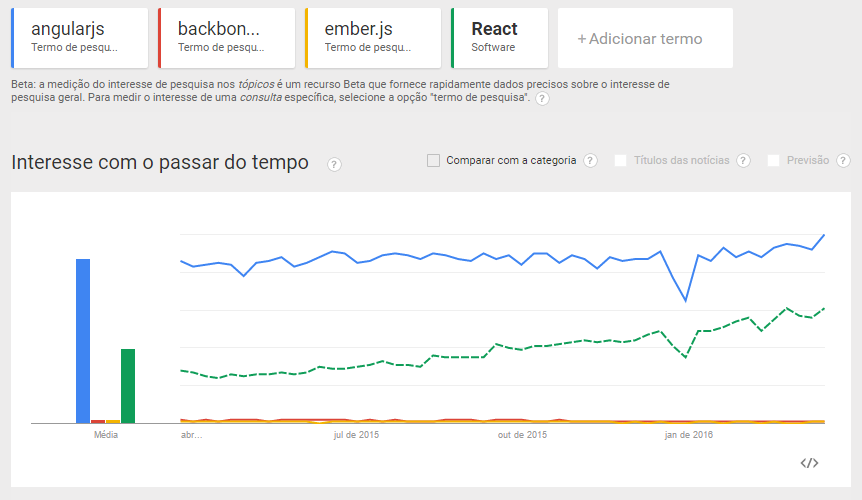
\includegraphics[width=1\textwidth]{img/grafico_ferramentas_front}
	\caption{Gráfico do Google Trends exibindo as pesquisas por ferramentas front-end}
\end{figure}


Junto ao Angular JS, será utilizada a agradável tendência de interface do Material Design da Google, que propõe layouts limpos e otimizados já conhecidos pelos usuários de smartphones Android. 


Para a elaboração da plataforma mobile do projeto, será utilizado o Ionic Framework, muito difundido e bastante pesquisado na área, o que fica evidenciado com o gráfico de pesquisa abaixo, coletado via Google Trends em \cite{GoogleTrends-Mobile-hybrid-Frameworks} buscando por frameworks de desenvolvimento híbrido mobile.


\begin{figure}
	\label{fig:graficoGoogleTrendsFerramentasHibridasMobile}
	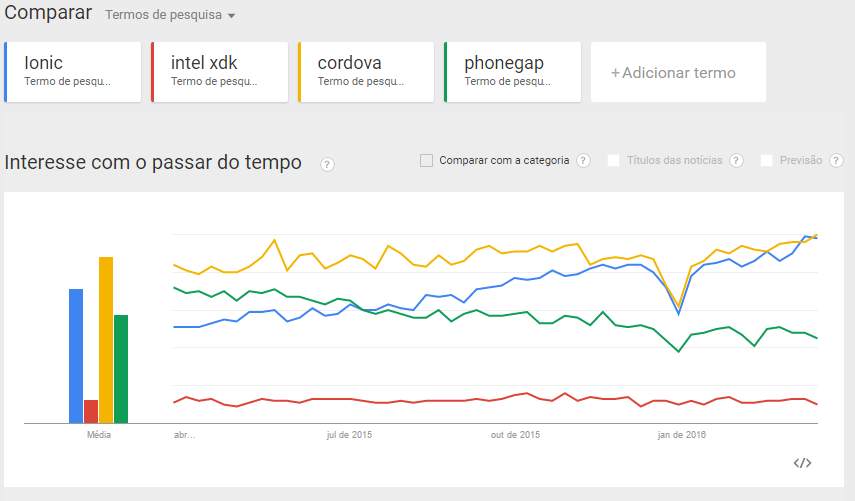
\includegraphics[width=1\textwidth]{img/grafico_ferramentas_hibridas_mobile}
	\caption{Gráfico do Google Trends exibindo as pesquisas por Frameworks híbridos mobile}
\end{figure}	

Para layout da interface mobile, também será aplicado a tendência do Material Design, a fim de propor uma harmonia entre o módulo web e mobile para os usuários


\section{Resultados Esperados}


Como fruto de um sistema para pós-graduação da UFBA, espera-se que os professores tenham mais recursos para integrar as atividades e também prover melhores condições para acompanhamento da vida acadêmica dos alunos em questão. Também, que os novos colaboradores que entrarem no processo tenham facilidade de compreender o fluxo do setor ao navegar pelo sistema proposto.


\section{Fora de Escopo}


Interação com os alunos devido às complicações para realizar a integração com o sistema empregado na UFBA, gerenciado pela XXXXXX, o que causaria uma inviabilidade no projeto devido à necessidade de entrega do produto ser mais forte que o tempo necessário para executar o processo de obtenção de acesso ao sistema legado para realizar a integração.


\section{Estrutura do Trabalho}


<breve resumo sobre os capítulos do TCC>